\documentclass[mathserif, aspectratio=169]{beamer}
%
%%%%%%%%%%%%%%%%%%%%%%%%%%%%%%%%%%%%%%%%%%%%%%%%%%%%%%%%%%%%%%%%%%%%%%%%
% need to split the includes to make spell checking work.
\usepackage{arev, arevmath}
\usepackage[scaled]{cabin}
\usepackage[T1]{fontenc}
\usepackage[super]{nth}
\usepackage{pifont}
\usepackage{wasysym}
\usepackage{tabularx}
\usepackage{array}
\usepackage{booktabs}
\usepackage{boldline}
\usepackage{colortbl}
%\usepackage{amsmath}
\usepackage{bm}
\usepackage{tcolorbox}
\usepackage{adjustbox}
\usepackage{minibox}
\usepackage{makecell}
\usepackage{adjustbox}
\usepackage{textcomp}
\usepackage[absolute,overlay]{textpos}
\setlength{\TPHorizModule}{1mm}%
\setlength{\TPVertModule}{1mm}%
\tcbuselibrary{skins}

\makeatletter
\newcommand{\antsize}{\@setfontsize{\antsize}{4pt}{4pt}}
\makeatother
\newcommand{\at}{\makeatletter @\makeatother}

\newcommand{\cmark}{\ding{51}}%
\newcommand{\bottomline}[1]{\vskip0pt plus 1fill{\alert{#1}\phantom{g}\vskip 1.0mm}}

\newcommand{\Quote}[2]{%
	\begin{center} 
		\begin{minipage}{0.7\textwidth} 
			\hrule
			\vskip 3mm
			\emph{{\color{ICTPblue} ``#1''}
			
			~~~~ {\color{ICTPorange} --- #2}}
			\vskip 3mm
			\hrule
			\vskip 2mm
		\end{minipage}
	\end{center}}


\mode<presentation>%
{
	\usetheme{default}
	%\usetheme[width=2.5cm]{PaloAlto}
	\usecolortheme{dove}
	\useoutertheme{infolines}
	% oder auch nicht

	% ICTP Colors
	\definecolor{ICTPblue}{RGB}{37,86,162} % 0x255682
	\definecolor{ICTPorange}{RGB}{255,130,0} % 0xff8200
	\definecolor{ICTPgreen}{RGB}{0,100,0}
	\definecolor{ICTPdark}{RGB}{80,80,80} % 0x505050
	\definecolor{ICTPlight}{RGB}{120,120,120}
	\definecolor{ICTPbrown}{RGB}{178,91,0}

	\definecolor{codebg}{rgb}{0.95,0.95,0.95}

	% Color theme
	\setbeamercolor{alerted text}{fg=ICTPorange}
	\setbeamercolor{frametitle}{fg=ICTPblue}
	\setbeamercolor{title}{fg=ICTPblue}
	\setbeamercolor{subtitle}{fg=ICTPorange}
	\setbeamercolor{normal text}{fg=ICTPdark}
	\setbeamercolor{author in foot}{fg=ICTPblue}
	\setbeamercolor{item}{fg=ICTPblue}
	\setbeamercolor{footline}{fg=ICTPblue}
	%\setbeamercolor{item projected}{bg=ICTPorange}
	%\setbeamercolor{item projected}{fg=white}

	\setbeamertemplate{headline}
	{}
	\setbeamertemplate{frametitle}
	{
		%\textbf{{\insertframetitle\phantom{g}}}\\
		%\textbf{\insertframetitle\phantom{g}}\\
		\textbf{\underline{\insertframetitle\phantom{g}}}\\
		%\textbf{\underline{\insertframetitle}}\\
		\vskip 1.0mm
		%{\color{UOLgold}\hrule height 2pt}
		%\par
	}
	\addtobeamertemplate{frametitle}{}{\vspace{-1em}}
	\setbeamertemplate{footline}{
		{%
			\textbf{ \hskip 3.0mm\insertshorttitle\phantom{.}---\phantom{.}\insertshortinstitute\hfill\insertframenumber\,/\,\inserttotalframenumber\hskip 3.0mm} 
		}
	}

	\setbeamertemplate{navigation symbols}{}%remove navigation symbols
	\setbeamertemplate{itemize items}[circle]
	\setbeamertemplate{enumerate items}[fg=ICTPblue]
	\setbeamercolor{itemize items}{fg=ICTPblue}
	\setbeamercolor{sidebar}{bg=ICTPblue}
	\setbeamercolor{title in sidebar}{fg=ICTPorange}
	\setbeamercolor{author in sidebar}{fg=ICTPorange}
	\setbeamercolor{section in sidebar}{fg=ICTPorange}
}

%\input{tikz/common-styles}

\usepackage{graphicx}
\usepackage[latin1]{inputenc}

\graphicspath{{../figs/}{../figs/common/}{../figs/islr/}}

\title[Statistical Learning] % (optional, nur bei langen Titeln n�tig)
{\textbf{Introduction to Statistical Learning\\ {\it with applications in Python}}\\%
		\href{www.statlearning.com}%
		{\tiny\it Based on ``Introduction to Statistical Learning, with applications in R'' by Gareth James, Daniela Witten, Trevor Hastie, Robert Tibishirani}\vspace{2em}}
		\vspace{-2.5cm}{}


		\author{\href{mailto:?to=Kurt Rinnert <kurt.rinnert@cern.ch>&subject=PWF Statistical Learning}{Kurt Rinnert}}

\institute[{\href{https://www.ictp.it/physics-without-frontiers.aspx}{Physics Without Frontiers} --- \href{https://www.ictp.it/}{ICTP}}] % (optional)
{\color{ICTPblue}\bfseries \href{https://www.ictp.it/physics-without-frontiers.aspx}{Physics Without Frontiers}\\\vspace{1mm}%
\href{https://www.ictp.it/}{
\includegraphics[width=0.20\textwidth]{common/ICTP-logo-full-trans.png}}\\%
\href{https://www.liverpool.ac.uk/physics/}{
\includegraphics[width=0.2\textwidth]{common/uol_logo.png}}}

\date{}

\titlegraphic{
	\texorpdfstring{\vspace{-2.8cm}}{}
	 \begin{minipage}[b][1.3cm][b]{0.26\textwidth}\color{ICTPlight}\antsize
		Copyright \textcopyright~2019\\
		\href{mailto:?to=Kurt Rinnert <kurt.rinnert@cern.ch>&subject=PWF Statistical Learning}{Kurt Rinnert <kurt.rinnert{\tt @}cern.ch>},
		\href{mailto:?to=Kate Shaw <kshaw@ictp.it>&subject=PWF Statistical Learning}{Kate Shaw <kshaw{\tt @}ictp.it>}\\
		Copying and distribution of this file, with or without modification,
		are permitted in any medium without royalty provided the copyright
		notice and this notice are preserved.  This file is offered as-is,
		without any warranty.


		Some of the figures in this presentation are taken from ``An Introduction to
		Statistical Learning, with applications in R''  (Springer, 2013) with
		permission from the authors: G. James, D. Witten,  T. Hastie and R. Tibshirani 
	 \end{minipage}\hspace{10cm}
}


\addtocounter{framenumber}{-1}

% nicer table row separation
\renewcommand{\arraystretch}{1.2}

% color boxes
\newcommand{\tabboxset}{\tcbset{enhanced, nobeforeafter, boxrule=0pt, boxsep=0pt, colback=codebg, colframe=codebg, coltext=ICTPdark, rounded corners, arc=4pt, fonttitle={\bfseries\tiny}}}
\newcommand{\codeboxset}{\tcbset{enhanced, nobeforeafter, boxrule=0pt, boxsep=0pt, colback=codebg, colframe=codebg, coltext=ICTPdark, rounded corners, arc=4pt, fonttitle={\bfseries\tiny}}}

\newcommand{\orange}{\color{ICTPorange}}
\newcommand{\blue}{\color{ICTPblue}}
\newcommand{\dark}{\color{ICTPdark}}
\newcommand{\R}{\mathbb{R}}
\newcommand{\dat}[1]{{\footnotesize\tt\orange #1}}
\newcommand{\e}[1]{\emph{#1}}
\newcommand{\bh}{\hat{\beta}}
\newcommand{\h}{\hat}

\makeatletter
\newcommand{\includegraphicsdpi}[3]{%
	\pdfimageresolution=#1%
	\includegraphics[#2]{#3}%
	\pdfimageresolution=72%
}

\newenvironment{blurb}%
	{\begin{center}\begin{minipage}{0.6\textwidth}\footnotesize}
	{\end{minipage}\end{center}}

\newenvironment{cpage}%
	{\begin{center}\begin{minipage}{0.75\textwidth}}
	{\end{minipage}\end{center}}

\newenvironment{popblock}[2]%
	{\begin{center}\begin{minipage}{#1}\footnotesize
		\begin{tcolorbox}[colframe=codebg, colback=white, colupper=ICTPdark, title={\normalsize\bfseries\blue #2}]}
	{\end{tcolorbox}\end{minipage}\end{center}}
\makeatother

\subtitle{\bfseries%
	{Classification}\\%
  {\tiny\it The classification scenario, Logistic Regression, Linear Discriminant Analysis, Quadratic Discriminant Analysis}\\%
}
\begin{document}
\frame[plain]{
	\vskip 1.0mm
	\titlepage
	\vskip 1.0mm
}


\begin{frame}{Abstract}
	\begin{blurb}
		In the regression scenario the response was quantitative. We now look into the 
		classification scenario in which the response is qualitative. 

		We will look at a few of the many available methods for classification in some detail.
		More methods will be covered in later lectures.
	\end{blurb}
\end{frame}

\begin{frame}{Overview}
	\begin{itemize}
		\item Classification versus Regression.
		\item Logistic Regression.
		\item Multiple logistic Regression.
		\item Linear Discriminant Analysis (LDA).
		\item Quadratic Discriminant Analysis (QDA).
	\end{itemize}
	\bottomline{Many ideas from the regression scenario will carry over.}
\end{frame}

\begin{frame}{Examples}
	\begin{itemize}
		\item Predicting a condition from symptoms in a hospital.
		\item Fraud detection in online payment systems.
		\item Predicting the probability of default on debt for credit card holders.
	\end{itemize}

	\bl{Classifications scenarios are very common.}
\end{frame}

\begin{frame}{Example: Default Data Set}
	\begin{center}
		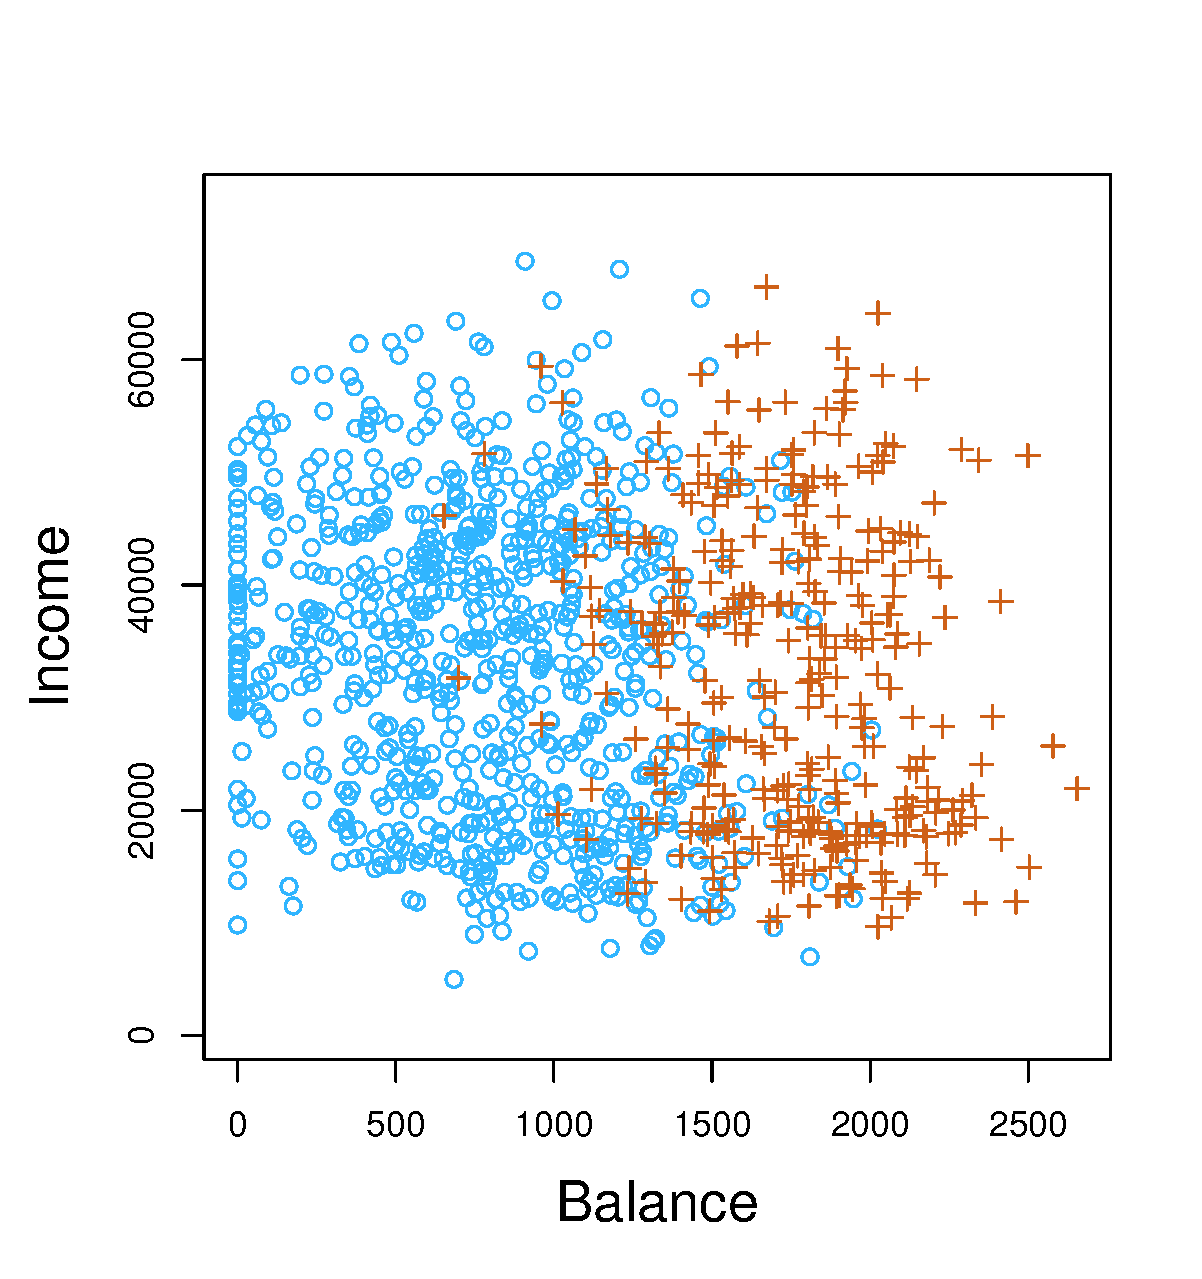
\includegraphics[width=0.34\textwidth]{4_1a}
		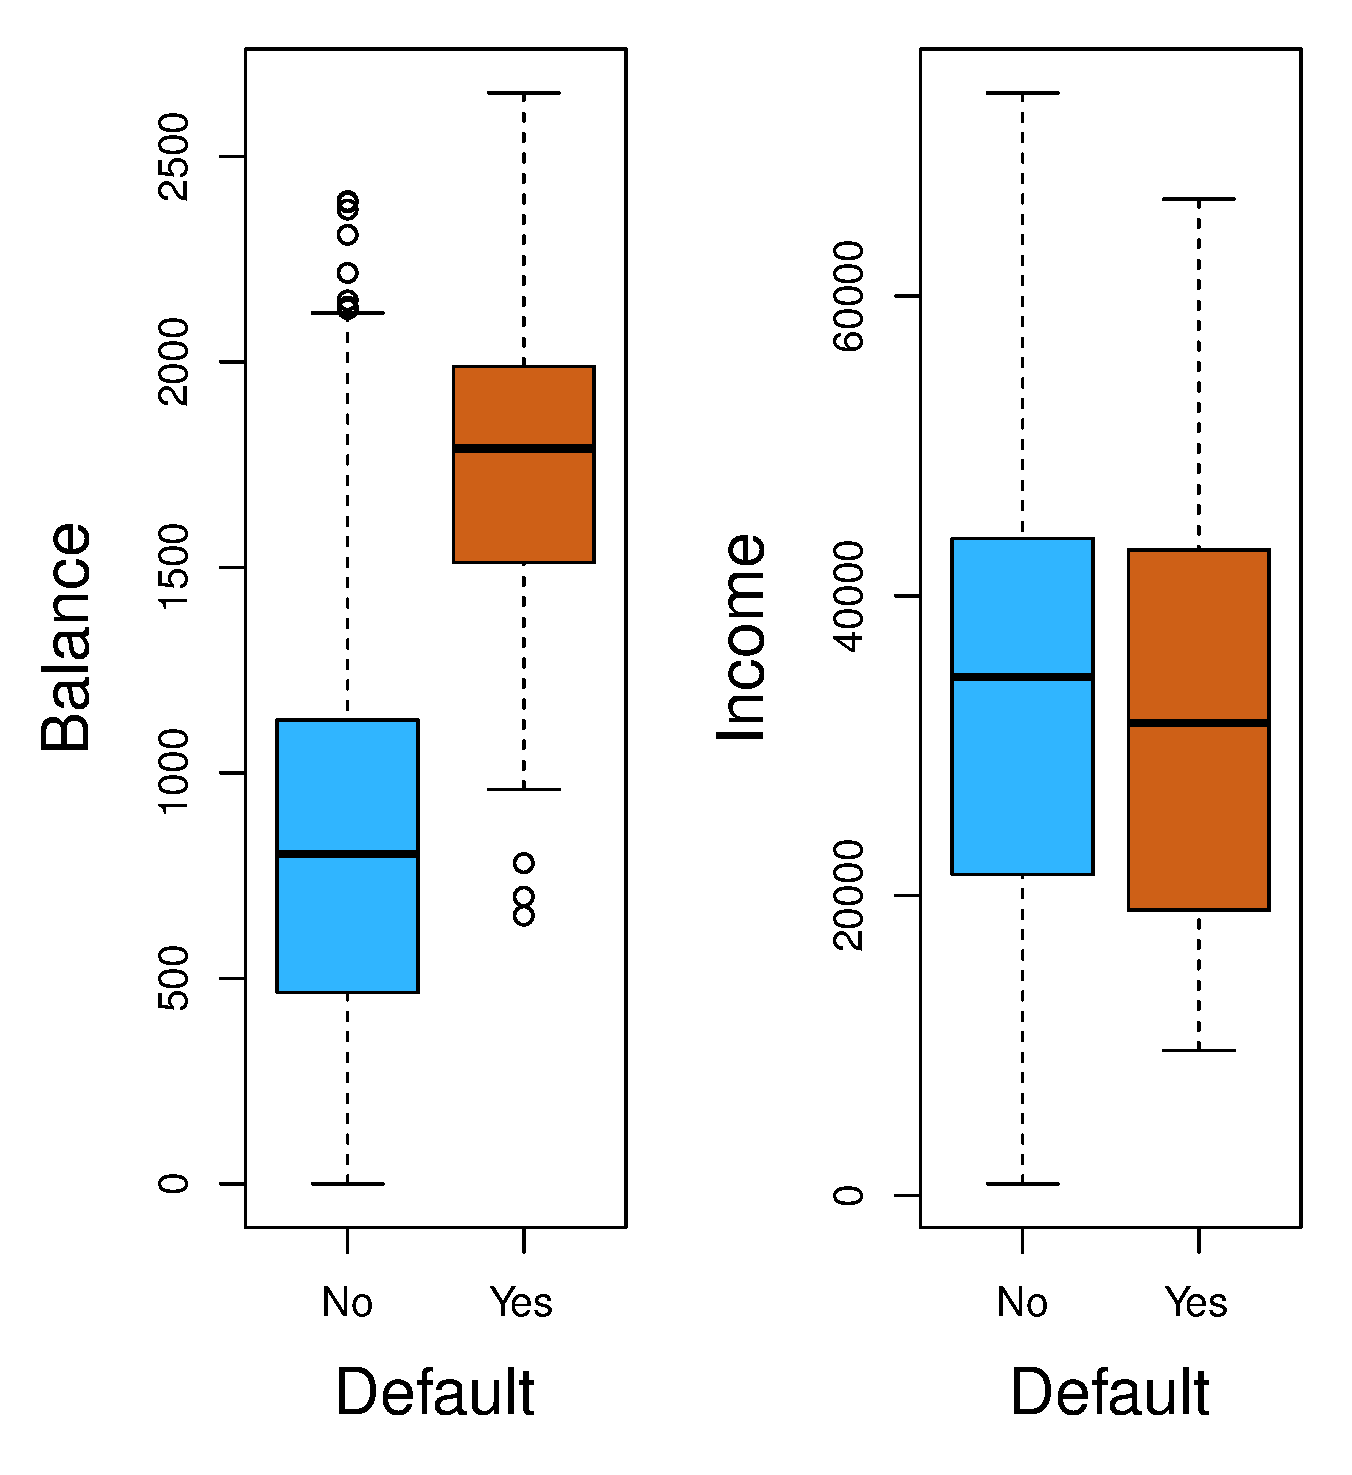
\includegraphics[width=0.3\textwidth]{4_1b}
	\end{center}

	Visualisation of the \dat{Default} data set. The classes are color coded.

	\bl{This is a simulated data set with an unusually high number of defaulters.}
\end{frame}

\begin{frame}{Example: Default Data Set}
	\begin{itemize}
		\item In this example the response is \e{binary}:
			\[
				y =
				\begin{cases}
					1 & \text{if \dat{default} is \val{Yes}} \\
					0 & \text{if \dat{default} is \val{No}} \\
				\end{cases}
			\]
		\item We encode qualitative responses the same way we encode qualitative predictors.
		\item Linear regression would work but is not ideal.
		\item \e{Logistic regression} is the superior method.
	\end{itemize}
	\bl{Logistic regression predicts probabilities.}
\end{frame}

\begin{frame}{Example: Default Data Set}
	\begin{itemize}
		\item For the \dat{Default} data set we would like to predict the probability
			of $\mdat{default} = \mval{Yes}$:
			\[ P(\mdat{default} = \mval{Yes} \vert \mdat{balance}) \]
		\item The probability is between $0$ and $1$.
		\item We can the \e{classify} based on $P$:
			\[ P(\mdat{default} = \mval{Yes} \vert \mdat{balance}) > 0.5\;:\; \mdat{default} = \mval{Yes} \]
	\end{itemize}
	\bl{we can of course choose different \e{working points}.}
\end{frame}

\begin{frame}{The Logistic Model}
	\begin{itemize}
		\item Out goal is to model the relationship
			\[ p(X) = P(Y=1\vert X) \leftrightarrow X \]
		\item We could use a linear regression model
			\[ p(X) = \beta_0 + \beta_1 X \]
		\item This does work but has some problems.
		\item In particular, the predicted probabilities can be $< 0$ or $> 1$.
	\end{itemize}
	\bl{We prefer a method that does not violate our axioms.}
\end{frame}

\begin{frame}{The Logistic Model}
	\begin{itemize}
		\item We must model $p(X)$ such that
			\[ p(X) \in \left[0, 1 \right] \;\;\forall X \]
		\item There a many functions that guarantee that.
		\item We use the \e{logistic function}
			\[ p(X) = \frac{e^{\beta_0 + \beta_1 X}}{ 1 + e^{\beta_0 + \beta_1 X}} \]
	\end{itemize}
	\bl{We will need a new fitting method for this.}
\end{frame}

\begin{frame}{The Logistic Model}
	\begin{center}
		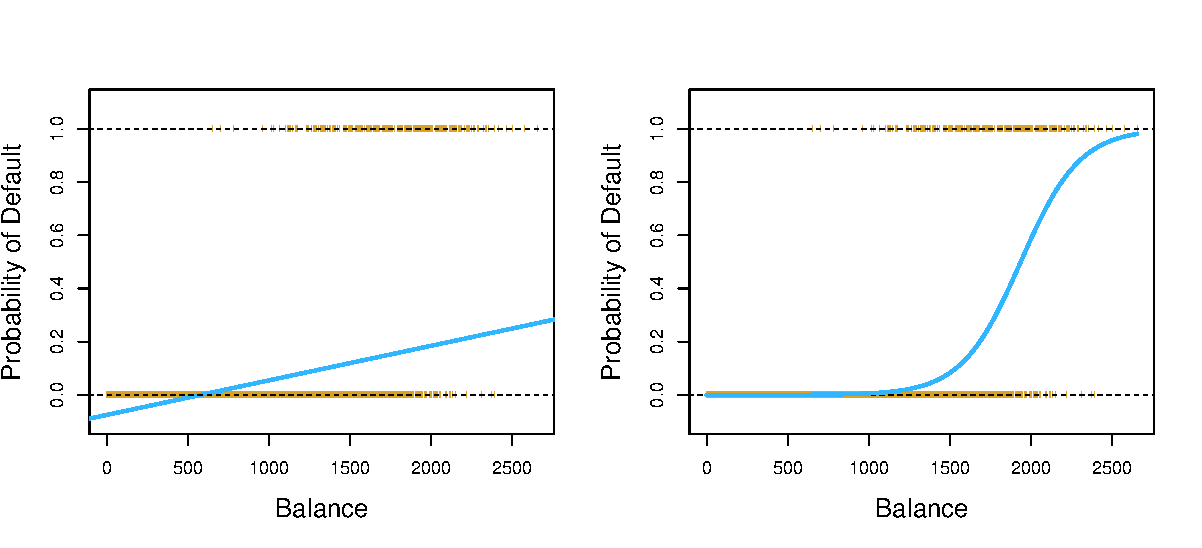
\includegraphics[width=0.8\textwidth]{4_2}

	Left: Linear Regression,
	Right: Logistic Regression
	\end{center}
	\bl{The logistic model satisfies our axioms.}
\end{frame}

\begin{frame}{The Logistic Model}
	\begin{itemize}
		\item The model looks complicated.
		\item How can we fit it?
		\item Some simple rearrangement yields the \e{odds}:
			\[ \frac{p(X)}{1 - p(X)} = e^{\beta_0 +\beta_1 X} \]
		\item For example:
			\[ p(0.2)\rightarrow\frac{1}{4}\;\;\;\;\text{and}\;\;\;\; p(0.9)\rightarrow 9 \]
	\end{itemize}
	\bl{Odds originate from betting on horse races.}
\end{frame}

\begin{frame}{The Logistic Model}
	\begin{itemize}
		\item How can the expression for the odds help us?
		\item How can we fit it?
		\item We take the logarithm of both sides to obtain
			\[ \log\left( \frac{p(X)}{1 - p(X)}\right)  = \beta_0 + \beta_1 X \]
		\item The left-hand side is called the \e{log odds} or \e{logit}.
	\end{itemize}
	\bl{The model for the logit is linear in $\bm{X}$.}
\end{frame}

\begin{frame}{The Logistic Model}
	\begin{itemize}
		\item  Recall that in linear regression $\beta_1$ describes the increase of $Y$ for
			a one-unit change in $X$.
		\item Here the interpretation is slightly more complicated.
		\item Changing $X$ by one unit changes the \e{logit} by $\beta_1$.
		\item Or equivalently, it multiplies the odds bt $e^{\beta_1}$.
		\item This does \e{not} imply a change of $\beta_1$ of $p(X)$!
		\item However, any \e{tendency} is preserved.
	\end{itemize}
	\bl{The logistic model has a nice interpretation.}
\end{frame}

\begin{frame}{Maximum Likelihood}
	\begin{itemize}
		\item Given
			\[ \log\left( \frac{p(X)}{1 - p(X)}\right)  = \beta_0 + \beta_1 X \]
			we could fit the logistic model with a linear lest square fit.
		\item  Instead, we will use a 
			\href{https://en.wikipedia.org/wiki/Maximum_likelihood_estimation}{\blue\underline{maximum likelihood}} fit.
		\item We have done this before without mentioning it.
	\end{itemize}
	\bl{Least Squares is just a special case of maximum likelihood.}
\end{frame}

\begin{frame}{Maximum Likelihood \& Bayes' Theorem}
	\vspace{-5mm}
	\begin{center}
		\[
			P(Y\vert X, I) = \frac{P(X\vert Y, I)\times P(Y\vert I)}{P(X\vert I)}
		\]
	\end{center}
	\begin{popblock}{0.4\textwidth}{}
		\begin{tabular}[h]{ll}
			\e{\blue\bfseries Term} & \e{\blue\bfseries Name} \\
			$P(Y\vert X, I)$ & posterior probability \\
			$P(X\vert Y, I)$ & likelihood \\
			$P(Y\vert I)$ & prior probability \\
			$P(X\vert I)$ & evidence \\
		\end{tabular}
	\end{popblock}
	\bl{We are going to derive the maximum likelihood method.}
\end{frame}

\begin{frame}{Maximum Likelihood \& Bayes' Theorem}
	\begin{itemize}
		\item We aim to produce the best estimate of $\bm{\beta}$.
		\item These are the \e{most probable} values of $\beta_0$ and $\beta_1$ 
			given the training data.
		\item That is, we seek to maximise
			\[ P(\bm{\beta}\vert X, I) \]
		\item A priori, we do not know how to construct this probability.
	\end{itemize}
	\bl{And here comes the power of Bayes' theorem\dots}
\end{frame}

\begin{frame}{Maximum Likelihood \& Bayes' Theorem}
	\begin{itemize}
		\item Given the training data \e{and} a model description we \e{can} construct the likelihood
			\[ P(X\vert\bm{\beta}, I) \]
		\item We can then use Bayes' theorem to obtain the posterior probability
			\[
				P(\bm{\beta}\vert X, I) = 
				\frac{P(X\vert\bm{\beta}, I) P(\bm{\beta}\vert I)}{P(X\vert I)}
			\]
		\item Or, up to a normalisation factor
			\[
				P(\bm{\beta}\vert X, I) \propto P(X\vert\bm{\beta}, I) P(\bm{\beta}\vert I)
			\]
	\end{itemize}
	\bl{All we need is a prior and we are all set.}
\end{frame}

\begin{frame}{Maximum Likelihood \& Bayes' Theorem}
	\begin{itemize}
		\item We choose the prior to reflect our knowledge (or rather lack thereof) \e{without}
			taking the training data into account.
		\item A good start is to assume complete ignorance.
		\item In many cases a good ignorant prior is a flat distribution:
			\[ P(\bm{\beta}\vert I) = \text{const.} \]
	\end{itemize}
	\bl{The influence of the prior quickly becomes negligible for large data sets.}
\end{frame}

\begin{frame}{Maximum Likelihood \& Bayes' Theorem}
	\begin{itemize}
		\item The uniform (constant) prior can be absorbed in the normalisation and we obtain
			\[ P(\bm{\beta}\vert X, I) \propto \underbrace{P(X\vert\bm{\beta}, I)}_\text{likelihood} \]
		\item In practice we often use the logarithm of the likelihood
			\[ \log\left( P(X\vert\bm{\beta}, I)\right) \] 
		\item Sometimes this allows for nice \& easy analytical solutions.
		\item More importantly in practice it is numerically much more stable.
	\end{itemize}
	\bl{Now maximising the likelihood does maximise the posterior!}
\end{frame}

\begin{frame}{Maximum Likelihood \& Bayes' Theorem}
	\begin{itemize}
		\item Under the assumption that the $x_i$ are independent we have
			\[ P(X\vert\bm{\beta}, I) = \prod_{i=1}^n P(x_i\vert\bm{\beta}, I) \]
		\item This follows from the product rule
			\[ P(x_i, x_k \vert\bm{\beta}, I) = P(x_i\vert x_k, \bm{\beta}, I) P(x_k\vert\bm{\beta}, I) \]
			and the independence assumption
			\[ P(x_i\vert x_k, \bm{\beta}, I) = P(x_i\vert\bm{\beta}, I) \]
	\end{itemize}
	\bl{We still need a model, though.}
\end{frame}

\begin{frame}{The Binomial Distribution}
	\begin{itemize}
		\item We need a model to describe a qualitative response variable with two classes (levels).
		\item The 
			\href{https://en.wikipedia.org/wiki/Binomial_distribution}{\blue\underline{binomial distribution}}
			describes this situation
			\[
				P(r\vert n, I) =
				\frac{n!}{n!(n - r)!}
				p^r (1 - p)^{n -r}
			\]
	\end{itemize}
	\bl{This is the probability to observe $\bm{r}$ ``successes''.}
\end{frame}

\begin{frame}{The Likelihood Function}
	\begin{itemize}
		\item We can now construct the \e{likelihood function} for the logistic regression:
			\begin{align*}
				P(X\vert\bm{\beta}, I) &= \prod_{i=1}^{n} P(x_i\vert\bm{\beta}, I) \\
				{} &= \prod_{y_i = 1} p(x_i) \prod_{y_i\neq 1} (1 - p(x_i))\\
			\end{align*}
			with
			\[ p(x_i) = \frac{e^{\beta_0 + \beta_1 x_i}}{ 1 + e^{\beta_0 + \beta_1 x_i}} \]
	\end{itemize}
	\bl{Different problems require different likelihood functions.}
\end{frame}

\begin{frame}{Maximum Likelihood Estimate}
	\begin{itemize}
		\item In practice we often us the logarithm of the likelihood function.
		\item The logarithm is a strictly monotonic function, so the extrema a preserved.
		\item Sometimes we minimise the negative logarithm.
		\item This is simply because of the abundance of minimisation libraries.
	\end{itemize}
	\bl{Wo do not care whether there is an analytical solution.}
\end{frame}

\begin{frame}{Logistic Regression Results}
	\begin{popblock}{0.7\textwidth}{}
		\begin{tabular}[h]{lrrrr}
			{} & {\blue Coefficient} & {\blue Std. Error} & {\blue $Z$-statistic} & {\blue $p$-value} \\
			\dat{Intercept} & $-10.6513$ & $0.3612$ & $-29.5$ & $< 0.0001$\\
			\dat{balance} & $0.0055$ & $0.0002$ & $24.9$ & $< 0.0001$\\
		\end{tabular}
	\end{popblock}
	\begin{itemize}
		\item Where the $Z$-statistic associated with $\beta_1$ is
			\[ Z = \frac{\bh_1}{\text{SE}(\bh_1)} \]
		\item For large samples the $Z$-statistic approaches the $t$-statistic.
	\end{itemize}
	\bl{In logistic regression we use the $\bm{Z}$-statistic and the associated $\bm{p}$-value.}
\end{frame}

\begin{frame}{Hypothesis Testing}
	\begin{itemize}
		\item The logistic null hypothesis is
			\[ H_0 : \beta_1 = 0 \implies p(X) = \frac{e^{\beta_0}}{1 + e^{\beta_0}} \]
		\item And the alternative hypothesis is
			\[ H_a : \beta_1 \neq 0 \implies p(X) = \frac{e^{\beta_0 + \beta_1 X}}
			{1 + e^{\beta_0 + \beta_1 X}} \]
	\end{itemize}
	\bl{We reject the null hypothesis based on a cut on the $\bm{p}$-value of the $\bm{Z}$-statistic.}
\end{frame}

\begin{frame}{A Word of Warning}
	\begin{itemize}
		\item The term ``maximum likelihood'' suggests that we have found the most probable values of 
			the parameters.
		\item This is in general \e{not} the case!
		\item We just determined the $\bm{\beta}$ that makes the \e{training data} most probable.
		\item It is important to keep this in mind.
		\item Consider the probability of rain given there are clouds versus the probability of clouds
			given it is raining.
	\end{itemize}
	\bl{In general $\bm{P(A\vert B) \neq P(B\vert A)}$.}
\end{frame}


\begin{frame}{Multiple Logistic Regression}
	\begin{itemize}
		\item We can generalise the logistic approach using the logit:
			\[
				\log\left( \frac{p(X)}{1 - p(X)}\right) =
				\beta_0 + \beta_1 X_1 + \dots + \beta_p X_P
			\]
			where
			\[ X = (X_1, \dots, X_p) \]
			are the $p$ predictors as ususal.
	\end{itemize}
	\bl{We start from the logit to stress the similarity to OLS.}
\end{frame}

\begin{frame}{Multiple Logistic Regression}
	\begin{itemize}
		\item We can easily translate this back to the logistic function:
			\[
				p(x) =
				\frac{e^{\beta_0 + \beta_1 X_1 + \dots + \beta_p Xp}}
				{1 + e^{\beta_0 + \beta_1 X_1 + \dots + \beta_p Xp}}
			\]
	\end{itemize}
	\bl{As in the simple case we use maximum likelihood.}
\end{frame}

\begin{frame}{Multiple Logistic Regression}
	\begin{popblock}{0.7\textwidth}{}
		\begin{tabular}[h]{lrrrr}
			{} & {\blue Coefficient} & {\blue Std. Error} & {\blue $Z$-statistic} & {\blue $p$-value} \\
			\dat{Intercept} & $-10.8690$ & $0.4923$ & $-22.08$ & $< 0.0001$\\
			\dat{balance} & $0.0057$ & $0.0002$ & $24.75$ & $< 0.0001$\\
			\dat{income} & $0.0030$ & $0.0082$ & $0.37$ & $0.7115$\\
			\dat{student[Yes]} & $-0.6468$ & $0.2362$ & $-2.74$ & $0.0062$\\
		\end{tabular}
	\end{popblock}
	\begin{itemize}
		\item The negative coefficient for \dat{student[Yes]} indicates that
			students are \e{less} likely to default.
		\item This holds fir \e{fixed values} of \dat{balance} and \dat{income}.
	\end{itemize}
	\bl{We should investigate this a bit further.}
\end{frame}

\begin{frame}{Multiple Logistic Regression}
	\vspace{-4mm}
	\begin{center}
		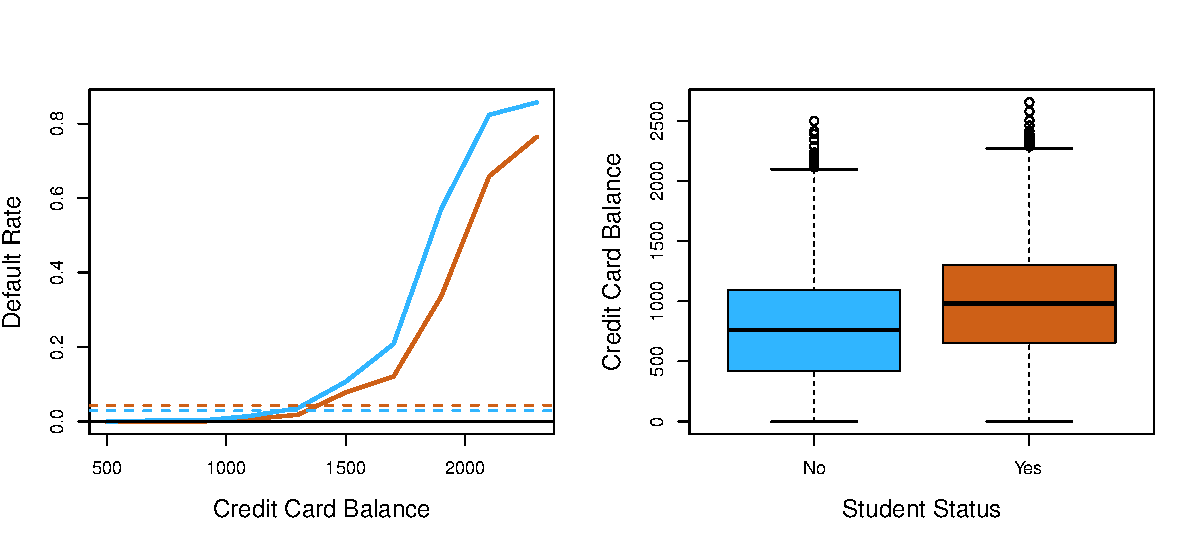
\includegraphics[width=0.7\textwidth]{4_3}
	\end{center}
	\begin{itemize}
		\item Students ({\orange orange}) and non-students ({\blue blue}).
		\item Solid lines: $\mdat{default} = f(\mdat{balance})$.
		\item Dashed: overall default rate.
		\item Students have a higher \dat{balance}.
	\end{itemize}
	\bl{There is a correlation!}
\end{frame}

\begin{frame}{The Bayes Classifier}
	\begin{itemize}
		\item Suppose we have $K$ classes with $K\ge2$.
		\item The we can specify the posterior probability as
			\[
				P(Y=k\vert X=x) =
				\frac{\pi_k f_k(x)}
				{\sum_{l=1}^K \pi_l f_l(x)}
			\]
			where $\pi_k$ is the prior and
			\[
				f_k(x) = P(X=x\vert Y=k)
			\]
		\item The problem now is the specification of $f_k$.
	\end{itemize}
	\bl{The Bayes classifier is the gold standard.}
\end{frame}

\begin{frame}{Linear Discriminant Analysis}
	\begin{itemize}
		\item For now we assume one predictor, that is $p=1$
		\item We want to find $f_k(x)$ in order to find $p_k(x)$.
		\item Once we have that, we can classify observations by choosing\\
			the class with the greatest $p_k(x)$.
	\end{itemize}
	\bl{We need to make some further assumptions about $\bm{f_k}$.}
\end{frame}


\begin{frame}{Linear Discriminant Analysis}
	\begin{itemize}
		\item We now also assume that $f_k(x)$ is \e{normal} (\e{Gaussian}).
		\item In the case of $p=1$ this means
			\[
				f_k(x) = \frac{1}{\sqrt{2\pi \sigma_k^2}}
				\exp\left(
				-\frac{1}{2\sigma_k^2}
				\left( x - \mu_k\right)^2
				\right)
			\]
		where $\mu_k$ and $\sigma_l$ may vary by class.
	\end{itemize}
	\bl{Even more assumptions follow\dots}
	
\end{frame}

\begin{frame}{Linear Discriminant Analysis}
	\begin{itemize}
		\item For now we further assume that
			\[ \sigma_1 = \sigma_2 = \dots = \sigma_K = \sigma \]
		\item This yields
			\[
				p_k(x) =
				\frac{\pi_k
					\exp\left(
					-\frac{1}{2\sigma^2}
					\left( x - \mu_k\right)^2
					\right)
				}{\sum_{l=1}^K\pi_l
					\exp\left(
					-\frac{1}{2\sigma^2}
					\left( x - \mu_l\right)^2
					\right)
				}
			\]
	\end{itemize}
	\bl{We assign the observation $\bm{X = x}$ to the class with the largest $\bm{p_k(x)}$.}	
\end{frame}


\begin{frame}{Linear Discriminant Analysis}
	\begin{itemize}
		\item By taking the logarithm, this is equivalent to choosing the class $k$ for which
			\[
				\delta_k(x) =
				x \frac{\mu_k}{\sigma^2} 
				- \frac{\mu_k^2}{2\sigma^2}
				+ \log\left(\pi_k\right)
			\]
			is largest.
		\item For example, if $K=2$ and $\pi_1 = \pi_2$, the Bayes classifier
			assigns:
			\[
				\text{class} =
				\begin{cases}
					1 & \text{if}\;\; 2x(\mu_1 - \mu_2) > \mu_1^2 - \mu_2^2\\
					0 & \text{otherwise}\\
				\end{cases}
			\]
	\end{itemize}
	\bl{In practice we don't have access to the true parameters.}
\end{frame}

\begin{frame}{Linear Discriminant Analysis}
	\begin{itemize}
		\item We have to \e{estimate} the parameters taking into account 
			our assumptions.
		\item LDA does just that and yields
			\begin{align*}
				\hat{\mu}_k &= \frac{1}{n_k}\sum_{y_i = k} x_i\\
				\hat{\sigma}^2 &= \frac{1}{n - K}
				\sum_{k=1}^{K}\sum_{y_i = k} (x_i - \hat{\mu}_k)^2\\
			\end{align*}
	\end{itemize}
	\bl{Let's talk about the interpretation.}
\end{frame}

\begin{frame}{Linear Discriminant Analysis}
	\begin{itemize}
		\item The estimate $\hat{\mu}_k$ is the average of all training observations
			of the $k$th class.
		\item The estimate $\hat{\sigma}^2$ is the weighted average of the sample
			variances of the $K$ classes.
		\item If we don't know the $\pi_!, \dots, \pi_k$ we estimate them from their
			frequencies in the training sample:
			\[ \hat{\pi}_k = \frac{n_k}{n} \]
		\item We can now construct $\hat{\delta}(x)$:
			\[
				\hat{\delta}_k(x) =
				x \frac{\hat{\mu}_k}{\hat{\sigma}^2} 
				- \frac{\hat{\mu}_k^2}{2\hat{\sigma}^2}
				+ \log\left(\hat{\pi}_k\right)
			\]
	\end{itemize}
	\bl{LDA is linear in the sense that $\bm{\hat{\delta}_k}$ is linear in $\bm{x}$}.
\end{frame}

\begin{frame}{Linear Discriminant Analysis}
	\begin{center}
		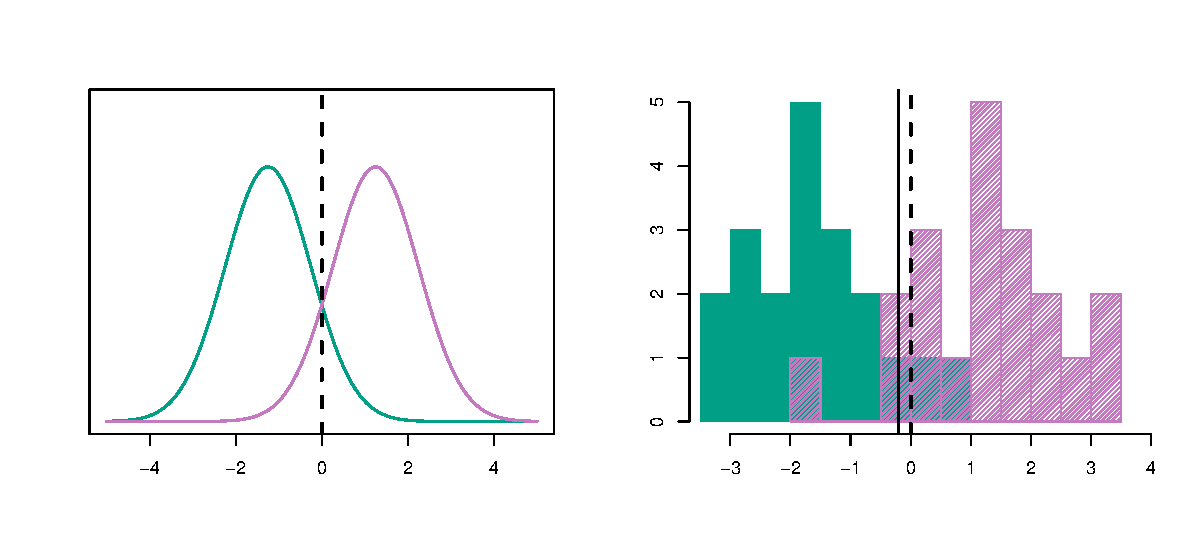
\includegraphics[width=0.8\textwidth]{4_4}
	\end{center}
	\bl{The error rate is only 0.5\%. LDA is doing well on this simulation.}
\end{frame}

\begin{frame}{LDA with $\bm{p > 1}$}
	\vspace{-10mm}
	\begin{center}
		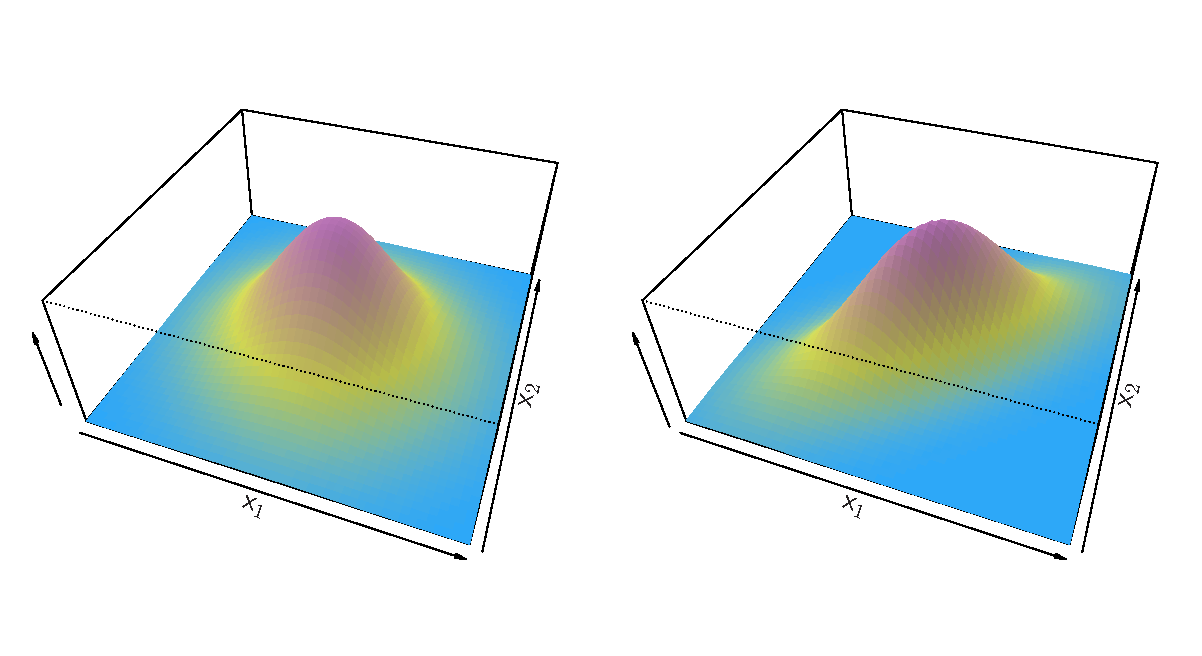
\includegraphics[width=0.8\textwidth]{4_5}
	\end{center}
	\vspace{-5mm}
	\begin{itemize}
		\item We now have a multivariate Gaussian distribution.
		\item We now have to estimate the covariance matrix $\bm{\Sigma}$.
	\end{itemize}
	\bl{Note that the variances can now be different.}
\end{frame}

\begin{frame}{LDA with $\bm{p > 1}$}
	\vspace{-10mm}
	\begin{center}
		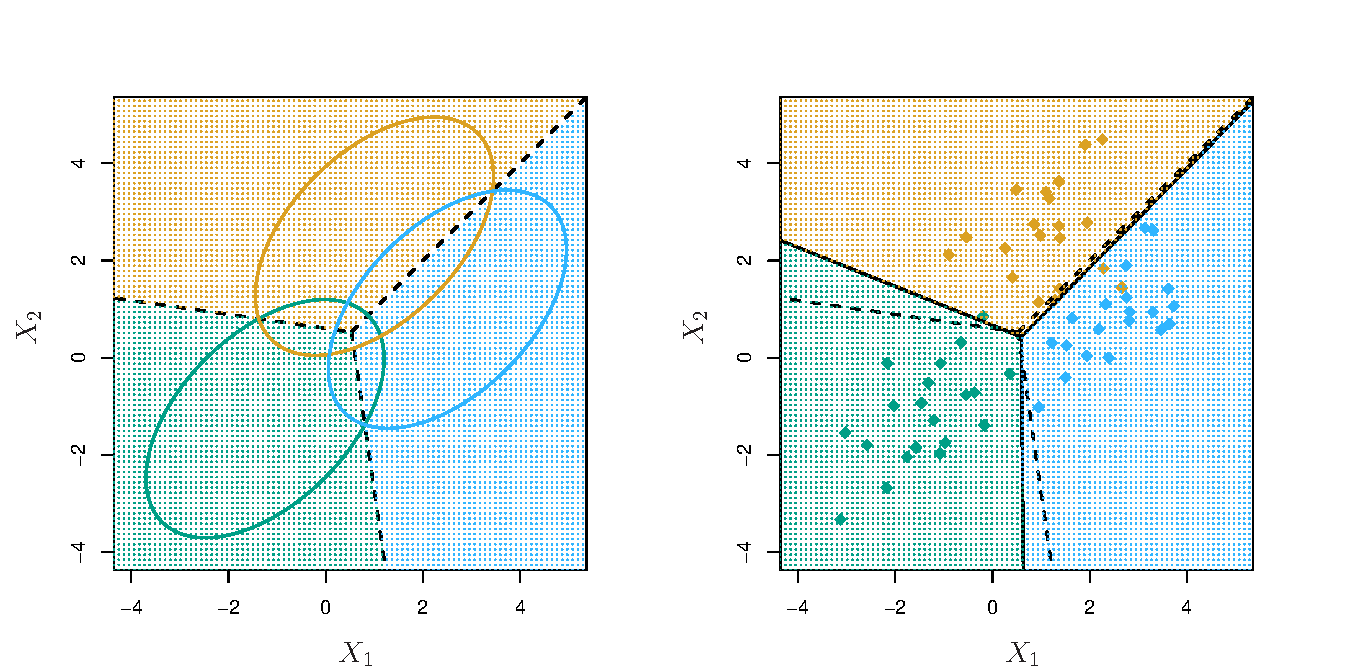
\includegraphics[width=0.8\textwidth]{4_6}
	\end{center}
	\vspace{-5mm}
	\begin{itemize}
		\item Dashed: Bayes decision boundary.
		\item Solid: LDA estimate.
	\end{itemize}
	\bl{This is a simulated example with three classes.}
\end{frame}

\begin{frame}{Quadratic Discriminant Analysis}
	\begin{itemize}
		\item QDA is an alternative approach to LDA that allows for curved boundaries.
		\item We drop the assumption that $\bm{\Sigma}$ is common to all classes.
		\item That means QDA provides an estimate $\bm{\hat{\Sigma}}_k$ in addition
			to $\hat{\mu}_k$ and $\hat{\pi}_k$.
	\end{itemize}
	\bl{The resulting $\bm{\hat{\delta}_k}$ is now quadratic in $\bm{x}$.}
\end{frame}

\begin{frame}{Quadratic Discriminant Analysis}
	\vspace{-10mm}
	\begin{center}
		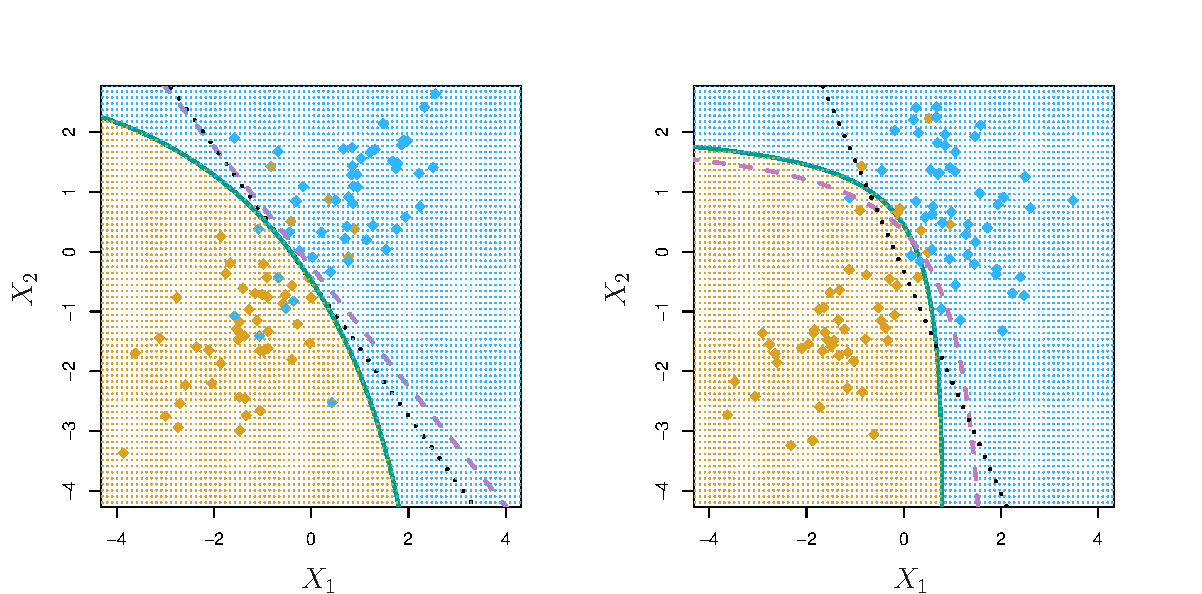
\includegraphics[width=0.8\textwidth]{4_9}
	\end{center}
	\vspace{-5mm}
	\begin{itemize}
		\item Left: $\bm{\Sigma}_1 = \bm{\Sigma}_2$
		\item Right: $\bm{\Sigma}_1 \ne \bm{\Sigma}_2$
	\end{itemize}
	\bl{The QDA performs better when the boundary is curved.}
\end{frame}

\begin{frame}{Classifier Performance}
	\vspace{-10mm}
	\begin{center}
		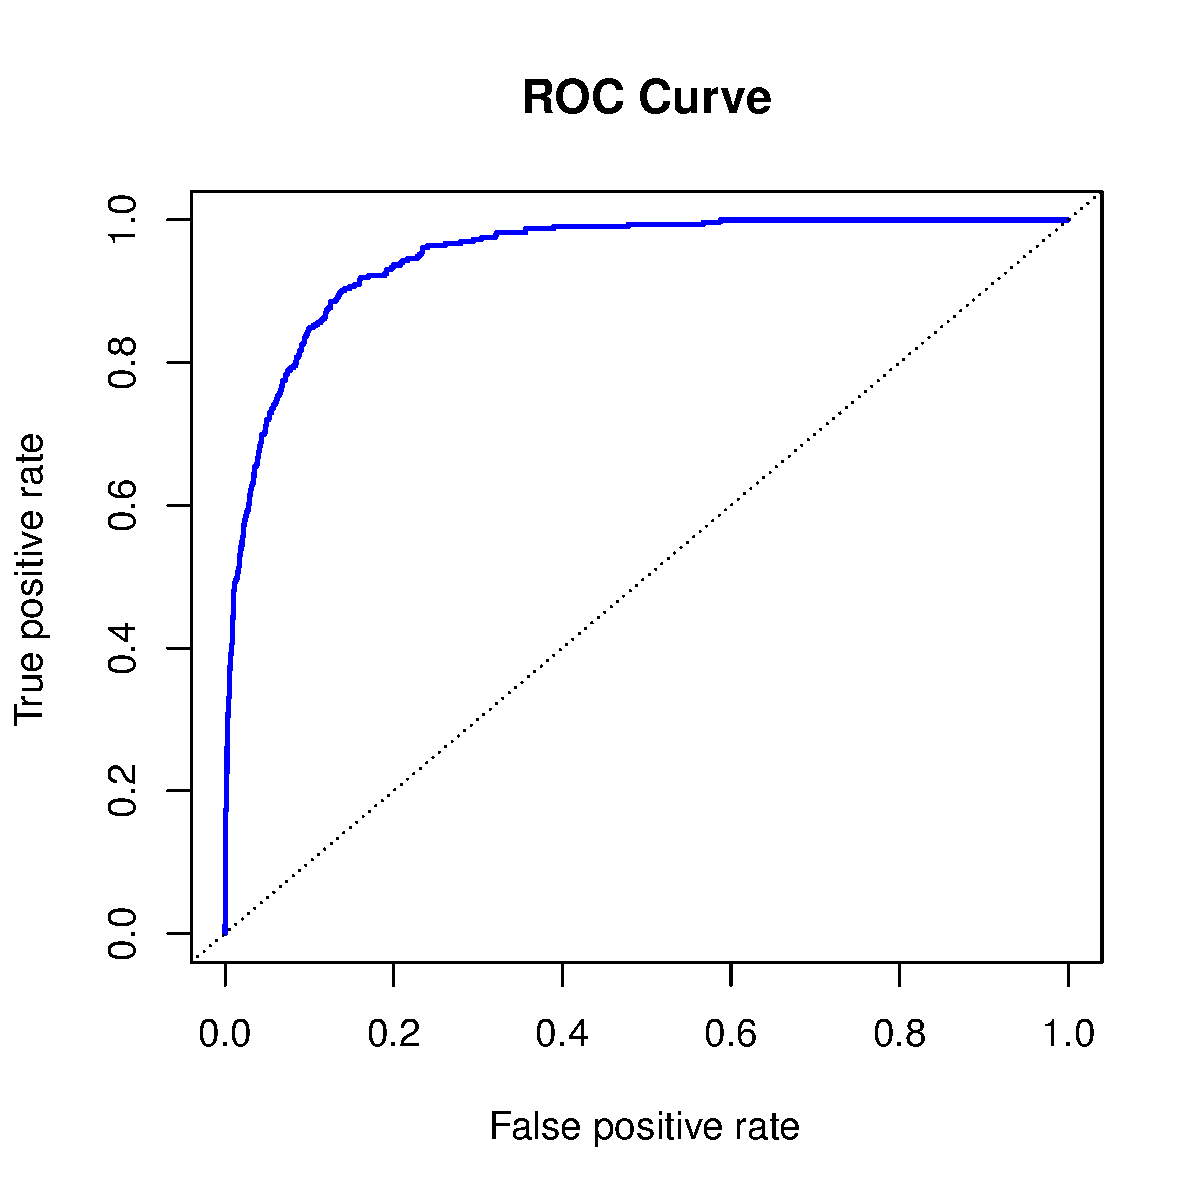
\includegraphics[width=0.55\textwidth]{4_8}
	\end{center}
	\vspace{-5mm}
	\bl{we can use this tho choose a \e{working point}.}
\end{frame}


\end{document}
